%%%%%%%%%%%%%%%%%%%%%%%%%%%%%%%%%%%%%%%%%%%%%%%%%%%%%%%%%%%%%%%%%%%%%%%
%
% Lignes de conduites
%
%%%%%%%%%%%%%%%%%%%%%%%%%%%%%%%%%%%%%%%%%%%%%%%%%%%%%%%%%%%%%%%%%%%%%%%

\subsection{Lignes de conduites}

Les pistes explorées par Ronan GOLHEN mettent en avant l'offre de
\textit{PaaS}\,\footnote{\textit{Plateform as a Service}, Plateforme
  en tant que service} Azure de \textit{Microsoft}. Les
caractéristiques principales de cette offre sont de libérer la société
de la gestion des serveurs et de ne payer qu'à l'usage, contrairement
aux offres \textit{IaaS}\,\footnote{\textit{Infrastructure as a
    Service}, Infrastructure en tant que Service}. Sa philosophie
incite fortement aux modèles de calcul parallèle.
%en effet on paye ici à l'utilisation, et non pour une période comme
%avec l'entretient de machines


Une architecture logicielle permettant de traiter une partie ou
l'ensemble de la production vecteur à l'intérieur du Cloud
\textit{Microsoft} doit être mise en place. Ce travail devra être
exploitable par les opérateurs de \textit{MapMedia} sans apprentissage
des technologies de développement.


%- moyens à mettre en œuvre.
%\subsection{Moyens à mettre en œuvre}
Migrer la chaine de production demande une bonne connaissance des
principes de workflow, de développement Azure et du Framework métier
\textit{OGR}.\\

Le workflow est à reconsidérer, on ne peut pas juste copier la chaine
existante pour deux raisons principales.

Tout d'abord le service hébergeur est distant et on ne peut pas se
permettre de controler toute la production dans les locaux, ce qui
impliquerait un rapatriment des données entre chacune de ces étapes
(plusieurs Giga-octets). 

Ensuite le fait que la chaine utilise des logiciels propriétaires pose
un problème de licence car ils sont liés à une machine physique,
principe à bannir en terme de technologie cloud.  Nous avons contacté
SAFE SOFTWARE, la société qui développe FME, cependant celle-ci n'est
pas prête à fournir des licences payantes au nombre
d'utilisateurs. Leur principe de licence prévoit que leur logiciel
doit s'exécuter toujours sur la même machine, chose inadaptée pour un
univers cloud.\\


Azure possède un Framework particulier qu'il faut maîtriser. Par
exemple les espaces de stockage permanent sont séparés des ressources
physiques de la machine, qui elles, deviennent des ressources
temporaires. Ainsi à chaque étape de calcul on sauvegarde les
résultats dans des espaces de stockage persistant appelé Azure Blob.\\

 \textit{OGR} sera la principale alternative à FME. En effet on doit
 pouvoir se passer de ce logiciel propriétaire et on peut se servir du
 Framework qu'il utilise puisque ce dernier est open source. Il a donc
 fallut refaire les étapes de production sans passer par
 l'intermédiaire de FME.\\






%%%%%%%%%%%%%%%%%%%%%%%%%%%%%%%%%%%%%%%%%%%%%%%%%%%%%%%%%%%%%%%%%%%%%%%
%
%   Plateforme Azure
%
%%%%%%%%%%%%%%%%%%%%%%%%%%%%%%%%%%%%%%%%%%%%%%%%%%%%%%%%%%%%%%%%%%%%%%%


%% Plus en Annexe ?

\subsection{Services fournit par la plateforme \textit{Windows Azure}}
Cette partie a pour but de familiariser le lecteur avec les concepts
Azure que nous emploierons plus tard. Nous allons évoquer des services
proposés par \textit{Microsoft}.\\


\subsubsection{Déploiement Azure}
L'offre de \textit{PaaS} Azure s'appuit principalement sur le fait de
déployer facilement des logiciels. Pour ce faire il faut développer un
code qui sera zippé dans un fichier de binaire et ressources
(extention \textit{.cspkg}) et un fichier de configuration (extention
\textit{.cscfg}). Un fois ces deux fichiers uploadés, via le portail
Azure\,\footnote{\textit{https://manage.windowsazure.com/}}, on peut
gérer notre déploiement. \\

\subsubsection{Worker Roles}
La cellule de base de l'architecture logicielle apportée est le Worker
Role, autrement dit le rôle de travail. \\

Lorsqu'on parle de worker role on fait souvent référence au code qui
le compose. L'unité de travail dans le déploiement Azure, qui
correspond à ce worker role, est une instance de ce worker role.  On
peut faire ici un parallèle avec un objet et une classe en
POO\,\footnote{Programmation Orientée Objet}.\\


Une implémentation de cette fonctionnalitée est fournit par
l'API\,\footnote{\textit{http://msdn.microsoft.com/en-us/library/microsoft.windowsazure.serviceruntime.roleentrypoint\_members.aspx}}. Il
s'agit d'une classe, C\# dans notre cas, nommée
\textit{RoleEntryPoint}. On peut créer une classe héritant de celle-ci
et redéfinir les méthodes $OnStart()$, $Run()$ et $OnStop()$. La
méthode la plus importante est la méthode $Run()$, on y met le code
que l'on veut exécuter.\\

Un worker role est censé tourner en boucle, ceci sans jamais
s'arrêter. Le processus peut tout de même s'interrompre dans des cas
particuliers. Si l'utilisateur décide de stopper son déploiement ou si
le rôle est transféré sur une autre machine alors la méthode
$OnStop()$ est appelée. Dans le cas d'un bug, bug du programme comme
la monopolisation de toutes les ressources ou bug externe comme une
coupure de courant, la méthode $OnStop()$ ne peut être appelée.\\

Le processus correspondant à une instance d'un worker role est exécuté
sur une VM\,\footnote{\textit{Virtual Machine}, Machine Virtuelle}
spécialement montée pour lui. On dispose sur cette machine, en
fonction des options de configuration, d'un certain espace mémoire et
d'une certaine quantité de mémoire disque. Les données enregistrées
sur le disque sont effacées avec l'interruption de la VM, lors de
l'arrêt de l'instance ou d'un dysfonctionnement du serveur. De plus
ces données sont locales à l'instance, les autres instances ne peuvent y
accéder.\\

%% TODO TODO TODO %%
%% TODO TODO TODO %%
%% TODO TODO TODO %%
%% TODO TODO TODO %%
%% TODO TODO TODO %%


Pour pouvoir sauvegarder des résultats accessibles par tous, y compris
pour les autres instances d'un même déploiement et utilisateurs
extérieurs, la plateforme Azure propose deux outils, l'Azure Storage
et Azure SQL.  On peut bien sur coder nos propres outils, qui upload
les données des instances sur un serveur de l'entreprise par
exemple. Cependant ces outils ont deux avantages majeurs. Ils sont
déjà fait et sont situés sur des machines proches des VM, d'un point
de vue géographique, ce qui augmente considérablement la bande
passante.\\


\subsubsection{Azure Storage}
Azure Storage est un espace de stockage de données numériques de
grande capacité. On y trouve trois services différents, les blobs, les
queues et les tables.\\

Les blobs sont des objets binaires non structurés, on peut les
assimiler à des fichiers. Ils sont regroupés dans des containers. On
peut assimiler les blobs à des fichiers et les containers à des
dossiers dans un système de fichier; à la différence qu'un container
ne peut pas posséder de containers. Les queues sont des files
FIFO\,\footnote{{First In First Out},Premier rentré premier sorti} de
messages, textes ou binaires. Elles implémentent plusieurs mécanismes
permettant de garantir la pérénité et la survie des messages. Les
tables sont des containers de données structurées, elle peuvent
contenir de nombreux objets de petite taille.\\



\subsubsection{Azure SQL}
Azure SQL est un serveur SQL hébergé dans des machines proches des
VM. Il s'agit en réalité d'un SQL Server légèrement modifié.\\



%%%%%%%%%%%%%%%%%%%%%%%%%%%%%%%%%%%%%%%%%%%%%%%%%%%%%%%%%%%%%%%%%%%%%%%
%
%   Archi globale ??
%
%%%%%%%%%%%%%%%%%%%%%%%%%%%%%%%%%%%%%%%%%%%%%%%%%%%%%%%%%%%%%%%%%%%%%%%

\subsection{Procédure de génération de cartes}

Pour produire les cartes au format dbv, l'opérateur utilisant la
solution créée pendant le stage doit faire quelques manipulations. \\

Il doit commencer par générer des tables SQL avec l'ancien système
(CATALOGUE\_RCL\_ALL, MX\_CHART, ...). Il les migre ensuite sur un
serveur \textit{SQL Azure}, grâce au logiciel \textit{SQL Database
  Migration Wizard}\,\footnote{Logiciel gratuit de migration de base
  de donnée, disponible sur sqlazuremw.codeplex.com}. De même grâce à
des logiciels comme \textit{Azure Storage Exploreur} ou
\textit{CloudBerry} les datas d'entrées, les cartes au format .s57, sont
placées dans des Blobs Azure.\\

Après avoir préparé un espace de travail Azure, il déploie la solution
sur le Cloud Azure. Une fois les instances de travail opérationnelles,
il peut utiliser les différents scripts, fichiers .bat, mis à sa
disposition pour exécuter les différentes étapes de la création du
dbv. Dans l'ordre ces étapes se nomment : Reprojection, MainProduction,
PostProduction1, PostProduction2 et Copie.\\

Enfin, il récupère les résultats obtenus (fichier dbv) à partir d'un
blob Azure.

% process générale pour produire des cartes



%\subsubsection{}

%\subsubsection{}

%\subsubsection{}






















%%%%%%%%%%%%%%%%%%%%%%%%%%%%%%%%%%%%%%%%%%%%%%%%%%%%%%%%%%%%%%%%%%%%%%%
%
%  Archi globale
%
%%%%%%%%%%%%%%%%%%%%%%%%%%%%%%%%%%%%%%%%%%%%%%%%%%%%%%%%%%%%%%%%%%%%%%%


\subsection{Détail de l'architecture et choix d'implémentation}%Architecture globale}
Pour accompagner la construction du projet au niveau architecture
logicielle deux réunions ont été organisées avec des participants
extérieurs à \maxsea. La première avec des responsables du
\textit{MCIA}\,\footnote{\textit{Mésocentre de Calcul Intensif
    Aquitain}} a surtout abouti sur des considérations théoriques sur
le cloud computing. Ces personnes ont davantage l'habitude de
travailler sur des offres \textit{IaaS} et sur des environnements
UNIX. La seconde fut à Paris avec un expert en architecture Azure de
Mircosoft France et deux employés de la société YSANCE, qui ont fait
un projet semblable au notre. Cette dernière fut plus concrète car les
participants avaient l'habitude de manipuler les API de Windows
Azure. \\




La solution apportée consiste en un déploiement et donc en une
solution C\# Visual Studio\,\footnote{\textit{IDE} (Integrated development
  Environment) de \textit{Mircosoft}.}.
 %% WARGING !!  Besoin de le dire? Première fois que ça apparait ?




\subsubsection{La classe \textit{WorkerRole}}
La classe \textit{Worker Role} constitue le point d'entrée du
programme, elle hérite d'ailleurs de \textit{RoleEntryPoint}. Celle-ci
va instancier n threads de travail, puis va entrer dans une boucle
infinie de surveillance de ces threads. La création de ces threads se
fait grâce à la classe \textit{Thread}. Ils instancient une classe
\textit{Worker}. La surveillance n'a pas été implémentée, elle
consiste à vérifier qu'il n'y a pas de fuite mémoire, pour au besoin
stopper ou relancer des threads de travail.


\subsubsection{La classe \textit{Worker}}
La classe \textit{Worker} sert à trouver et répartir les tâches de
travail. Dans son instanciation elle créé dynamiquement, en utilisant
la réflexivité, un tableau d'objet héritant de la classe
abstraite \textit{BusinessProcess} et implémentant l'interface
\textit{IBusinessProcess}. Cette interface demande d'implémenter deux
méthodes, à savoir \textit{Init()} et \textit{Work()}. La seconde
renvoie $false$ si l'objet ne trouve pas de travail et $true$ après
avoir traité une tâche sinon. L'objet \textit{Worker} bouclera sur le
tableau pour que toutes les tâches soient traitées.

\begin{figure}[h!]
  \caption{Diagramme de classe partiel du Worker Role.}
  \centering
    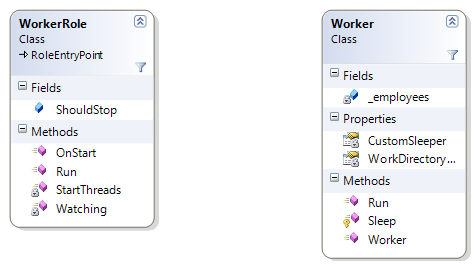
\includegraphics[width=0.8\textwidth]{images/WorkerRole.png}
\end{figure}

\subsubsection{Les classes héritant de \textit{BusinessProcess}}
Celles-ci se comportent globalement de la même manière. Lors de son
instanciation ou de l'appel à \textit{Init()} un objet héritant de
\textit{BusinessProcess} met en place son environnement de travail, et
crée notamment des chaines de connexion. Ensuite lors de l'appel à la
méthode \textit{Work} il vérifie si il a une tâche à faire. La plupart
du temps la liste des tâches est implémentées gràce à un objet
\textit{CloudQueue} de l'API Azure. \\

Si une tâche est trouvée alors la commande est interpretée à l'aide de
la classe \textit{CommandLine} et les fichiers nécessaires sont
ramenés des blobs Azure sur la VM (en local) afin de travailler avec.\\

Une fois cette étape de mise en place terminée, le code métier est
appelé. Il écrit soit directement les résultats dans une table SQL
Azure, soit dans un fichier qui sera ensuite remis dans un blob Azure.
Enfin le message correspondant à la tâche est supprimé.

\begin{figure}[h!]
  \caption{Diagramme des classes héritant de BusinessProduction.}
  \centering
    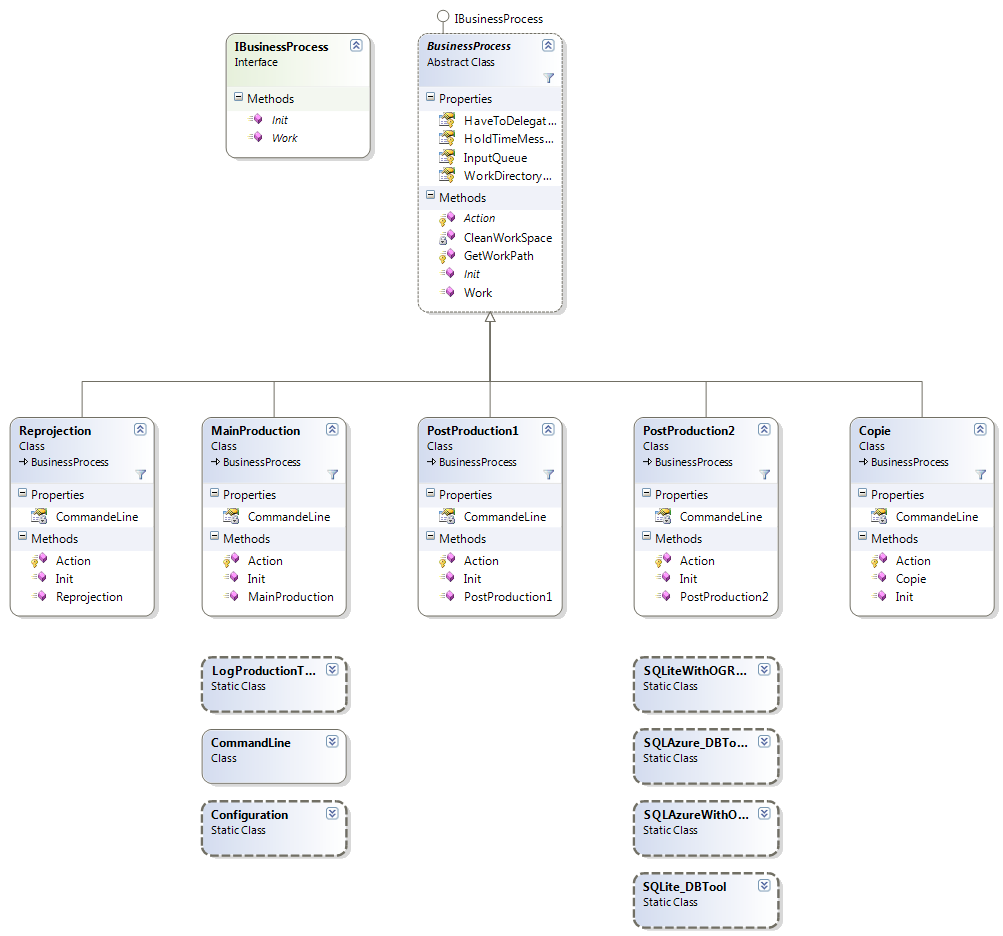
\includegraphics[width=0.8\textwidth]{images/BusinessProduction2.png}
\end{figure}
\subsubsection{La classe \textit{Manager}}

Un autre Worker Role nommé \textit{Manager} sert à générer les
milliers de messages envoyés aux queues de travail. C'est un processus
similaire au premier. \\

La classe \textit{WorkerRole} sert de point d'entrée, mais cette fois
il n'y a pas de thread de travail et de thread de
surveillance. L'objet instanciera directement un tableau d'objets
héritant de \textit{Manager} et implémentant l'interface
\textit{IManager}. Il boucle ensuite sur ce tableau pour savoir si il
existe des tâches à effectuer. Ces tâches sont différentes des
précédentes puisqu'il s'agit de créer des messages et de remplir des
queues.

\begin{figure}[h!]
  \caption{Diagramme de classe du Worker Role Manager.}
  \centering
    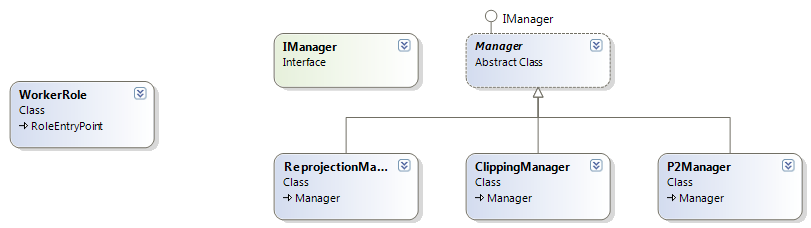
\includegraphics[width=0.8\textwidth]{images/Manager.png}
\end{figure}


%\subsubsection{}







%%%%%%%%%%%%%%%%%%%%%%%%%%%%%%%%%%%%%%%%%%%%%%%%%%%%%%%%%%%%%%%%%%%%%%%
%
% Travail métier
%
%%%%%%%%%%%%%%%%%%%%%%%%%%%%%%%%%%%%%%%%%%%%%%%%%%%%%%%%%%%%%%%%%%%%%%%

\subsection{Détails des tâches métiers}
Nous allons ici aborder les fonctionnalités métiers. \\ Elles se
séparent en 3 catégories. Les premières peuvent s'exécuter en
parallèle par carte, les secondes par RCL\,\footnote{\textit{Row
    Column Level}, Ligne Colone Niveau, méthode d'agencement en
  "quadtree pyramid"}. Pour la dernière catégorie le parallèlisme est
moins évident à mettre en place. \\

%A là fin d'une tâche, un message peut être automatiquement générer
%pour la suivante en mettant l'option "fullProduction" à $true$.

\subsubsection{La classe \textit{Reprojection}}
Message d'entrée : 
-inputcontainer:\textless \textit{input\_container\_name}\textgreater \   
-inputfile:\textless \textit{input\_file\_name}\textgreater \ 
[-outputContainer:\textless \textit{output\_container\_name} \textgreater ]\  
[-outputfile:\textless \textit{output\_file\_name}\textgreater ] \ 
[-fullProduction: $\{true;false\}$] \ 
-serveur:\textless \textit{server\_name}\textgreater \   
-dataBase:\textless \textit{data\_base\_name}\textgreater \   
-user:\textless \textit{user\_name}\textgreater  \ 
-pwd:\textless \textit{password}\textgreater  \ 
[-overwrite:$\{true;false\}$] \ 
[-update:$\{true;false\}$] \ 
-refFournisseur:\textless \textit{int\_provider}\textgreater \\   

Au départ d'une production nous possédons des fichiers .s57 dans un
container et des tables dans une base de donnée SQL Azure.  \\

Le fichier .s57 est ouvert avec l'API Ogr. Chaque ligne de la base de
donnée est ensuite recopiée dans un fichier sqlite en reprojetant
chaque coordonnée spatiale dans un autre référenciel spatial. Les
tables OBJECT\_TYPE, PROVIDER\_REFERENCE, CHART\_FID, CHART et
S57\_OBJECT sont créées et les trois premières remplies. Le résultat
est stocké dans un blob.


\subsubsection{La classe \textit{MainProduction}}
Message d'entrée : 
-inputcontainer:\textless \textit{input\_container\_name}\textgreater \   
-inputfile:\textless \textit{input\_file\_name}\textgreater \ 
[-outputContainer:\textless \textit{output\_container\_name} \textgreater ]\  
[-outputfile:\textless \textit{output\_file\_name}\textgreater ] \ 
-serveur:\textless \textit{server\_name}\textgreater \   
-dataBase:\textless \textit{data\_base\_name}\textgreater \   
-user:\textless \textit{user\_name}\textgreater  \ 
-pwd:\textless \textit{password}\textgreater  \ 
[-overwrite:$\{true;false\}$] \ 
[-update:$\{true;false\}$] \ 
[-jobToDo:{clipping;trinagulation;display3d}] \ 
[-layers:{all;\textless \textit{layers\_names} \textgreater} ] \\ 

Le fichier précédent est modifié par cette classe. Les géométries des
objets sont découpées, on parlera par la suite de clipping, selon la
table CATALOGUE\_RCL\_ALL et placées dans la table
CLIPPING\_OBJECT. Les géométries de type polygone obtenues sont
triangulées en utilisant les bibliothèques j3d\,\footnote{Java 3d, dll
  wrapée} et stockées dans la table TRIANGULATION\_2D. Enfin on calcul
un point d'affichage pour chaque géométrie, une sorte de barycentre
pour l'affichage. Ce résultat est distribué dans les tables
DISPLAY\_3D, DISPLAY\_3D\_POLYGONE, DISPLAY\_3D\_LINE.




\subsubsection{La classe \textit{PostProduction1}}
Message d'entrée : 
-inputcontainer:\textless \textit{input\_container\_name}\textgreater \   
-inputfile:\textless \textit{input\_file\_name}\textgreater \ 
[-outputContainer:\textless \textit{output\_container\_name} \textgreater ]\  
[-outputfile:\textless \textit{output\_file\_name}\textgreater ] \ 
[-fullProduction: $\{true;false\}$] \ 
-serveur:\textless \textit{server\_name}\textgreater \   
-dataBase:\textless \textit{data\_base\_name}\textgreater \   
-user:\textless \textit{user\_name}\textgreater  \ 
-pwd:\textless \textit{password}\textgreater  \ 
[-overwrite:$\{true;false\}$] \ 
[-update:$\{true;false\}$] \\ 

Dans les deux post-productions le système de traitement d'une tâche
est un peu plus complexe car on fait appel à un exécutable, le
\textit{displayStyler}, qui est une version modifiée pour l'occasion,
d'un code déjà existant et fonctionnel de l'entreprise. L'intégration
de ce code directement dans le code produit durant le stage pose des
problèmes de compatibilité de framework Microsoft. C'est pourquoi le
choix de modifier les sources de l'exécutable pour qu'il manipule
lui-même les objets Azure a été fait.\\

La première post-production travail encore par carte. Elle remplie les
tables CHART et S57\_OBJECTS avec des binaires représentant les
données des objets découpés.


\subsubsection{La classe \textit{PostProduction2}}
Message d'entrée : 
-inputcontainer:\textless \textit{input\_container\_name}\textgreater \   
-inputfile:\textless \textit{input\_file\_name}\textgreater \ 
[-outputContainer:\textless \textit{output\_container\_name} \textgreater ]\  
[-outputfile:\textless \textit{output\_file\_name}\textgreater ] \ 
[-fullProduction: $\{true;false\}$] \ 
-serveur:\textless \textit{server\_name}\textgreater \   
-dataBase:\textless \textit{data\_base\_name}\textgreater \   
-user:\textless \textit{user\_name}\textgreater  \ 
-pwd:\textless \textit{password}\textgreater  \ 
[-overwrite:$\{true;false\}$] \ 
[-update:$\{true;false\}$] \ 
-refFournisseur:\textless \textit{int\_provider}\textgreater \   
[-jobToDo:{clipping;trinagulation;display3d}] \ 
[-layers:{all;\textless \textit{layers\_names} \textgreater} ] \\

La seconde post-production travaille par RCL, ce qui oblige à
télécharger toutes les cartes sqlite du RCL. Une petite particularité
afin d'alléger les tables SQL Azure, ici les binaires générés sont
stockés dans des blob Azure et leurs références sont insérées dans les
tables RCL et S52\_RCL. Ces deux tables ne sont plus dans un fichier
sqlite mais bien sur SQL Azure afin de pouvoir gérer le parallèlisme à
gros grain facilement.

\subsubsection{La classe \textit{Copie}}
Message d'entrée : 
-inputcontainer:\textless \textit{input\_container\_name}\textgreater \   
-inputfile:\textless \textit{input\_file\_name}\textgreater \ 
[-outputContainer:\textless \textit{output\_container\_name} \textgreater ]\  
[-outputfile:\textless \textit{output\_file\_name}\textgreater ] \ 
[-fullProduction: $\{true;false\}$] \ 
-serveur:\textless \textit{server\_name}\textgreater \   
-dataBase:\textless \textit{data\_base\_name}\textgreater \   
-user:\textless \textit{user\_name}\textgreater  \ 
-pwd:\textless \textit{password}\textgreater  \ 
[-overwrite:$\{true;false\}$] \ 
[-update:$\{true;false\}$] \ 
-refFournisseur:\textless \textit{int\_provider}\textgreater \   
[-jobToDo:{clipping;trinagulation;display3d}] \ 
[-layers:{all;\textless \textit{layers\_names} \textgreater} ] \\

La dernière étape n'est pas parallèlisée. Elle s'appuie encore sur le
\textit{DisplayStyler}. Elle consiste grossièrement à regrouper tous
les résultats précédents en un seul fichier.




%%%%%%%%%%%%%%%%%%%%%%%%%%%%%%%%%%%%%%%%%%%%%%%%%%%%%%%%%%%%%%%%%%%%%%%
%
% Résultat 
%
%%%%%%%%%%%%%%%%%%%%%%%%%%%%%%%%%%%%%%%%%%%%%%%%%%%%%%%%%%%%%%%%%%%%%%%

\subsection{Résultats}

\subsubsection{Fichier au format dbv}

Un fichier dbv crée par la nouvelle chaine de production a pu être
lu par le logiciel MaxSea TimeZero. La migration de la chaine de
production est donc techniquement possible. Seul bémole à cet essai,
par manque de temps un seul rcl a été traité. Même si de nombreuses
étapes ont été testées en quantité (jusqu'à la post-production2), un
plus gros lots de rcl et de cartes pour la copie aurait été souhaitable.

\begin{figure}[h!]
  \caption{Rendu dans MaxSeaTZ d'un RCL produit sur le Could.}
  \centering
    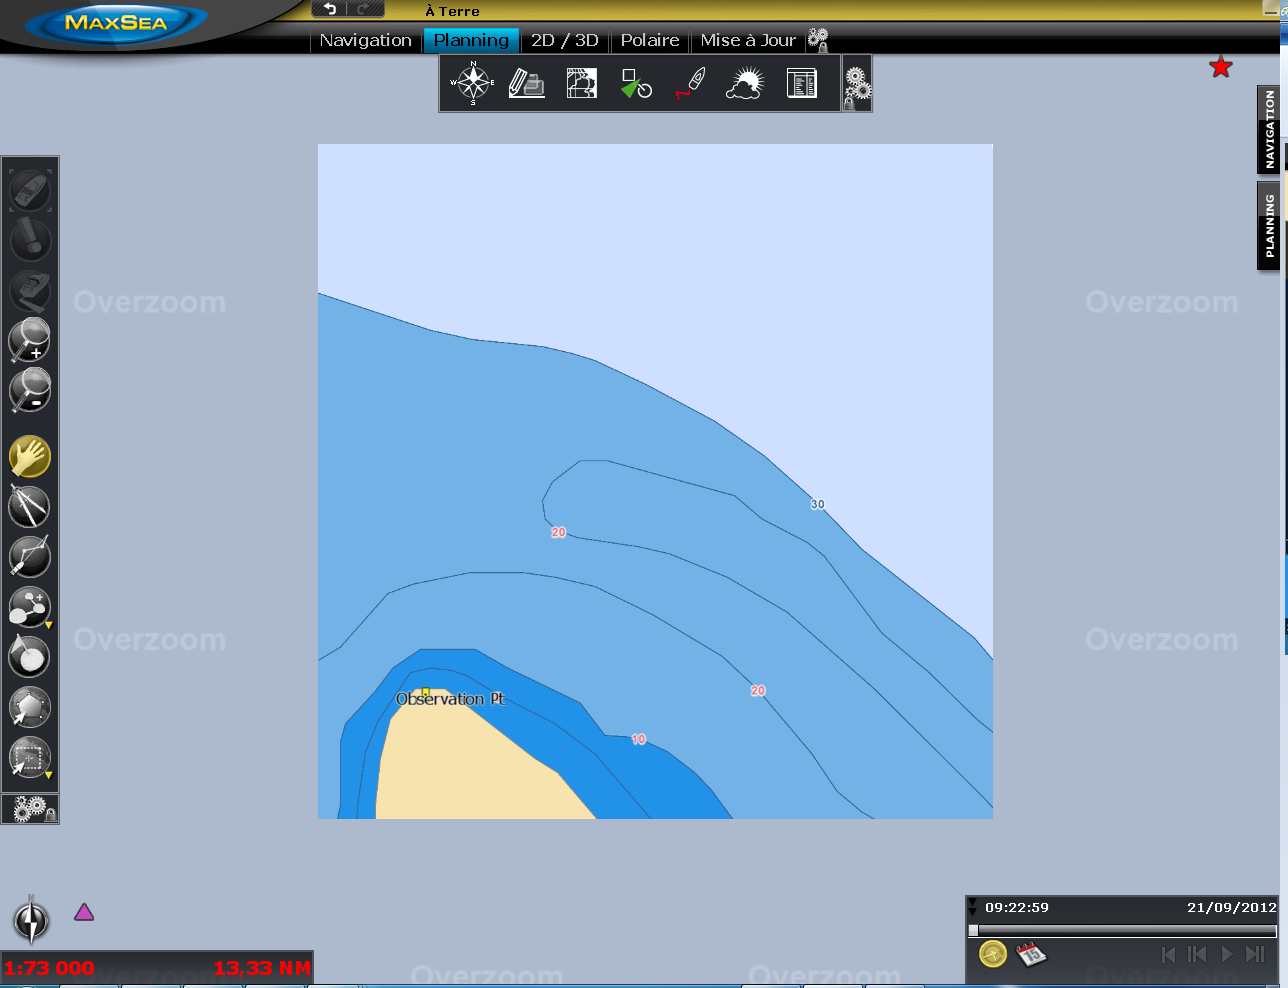
\includegraphics[width=0.8\textwidth]{images/rcl_L10_R799_C146.png}
\end{figure}

%%%%%%%%%%%%%%%%%%%%%%%%%%%%%%%%%%%%%%%%%%%%%%%%%%%%%%%%%%%%%%%%%%%%%%%
%
% Perf
%
%%%%%%%%%%%%%%%%%%%%%%%%%%%%%%%%%%%%%%%%%%%%%%%%%%%%%%%%%%%%%%%%%%%%%%%

%\subsection{Pérformances}

%Nous allons ici aborder les différents choix technique
%d'implémentation. %Point par point.

\subsubsection{Performance de travail}
La performance n'a pas été le facteur décisif. Cependant on peut dire
qu'on bénéficie avec ce système d'une bonne accélération, ou speed-up,
même si l'algorithme est loin d'être optimal. En effet trop de temps
est perdu dans les communications, en particulier dans le
téléchargement de fichiers sqlite. On remarque que, comme attendu, le
temps de production d'un lot donné est inversement proportionnel au
nombre de worker role, du moins pour les premières étapes pour
lesquelles des tests ont été effectués.

\subsubsection{Budgétaires}
La question du coût reste assez floue. En effet on ne peut pas faire
de comparatif entre les coûts de l'ancien système et ceux de la
production cloud. Nous ne disposons pas d'une estimation du coût
annuel de l'infrastructure dédiée à la production vecteur dans les
locaux de \maxsea car ces machines sont utilisées pour de nombreuses
fonctions simultanément. De plus seul un essai grandeur nature de bout
en bout peut vraiment nous donner le coût d'une production vecteur en
environnement cloud.


